\documentclass[10pt,a5paper]{article}
\renewcommand{\baselinestretch}{1.0}
\usepackage{cite}
\usepackage[dvips]{graphicx}
\usepackage{psfrag}
\usepackage{color}
\usepackage[cmex10]{amsmath}
\usepackage{amsfonts}
\usepackage[font=footnotesize, captionskip=10pt]{subfig}
\usepackage{tikz}
\usepackage{flushend}
\usepackage{times}
\usepackage[margin=1.5cm]{geometry}
\pagestyle{empty}

\hyphenation{net-works}
\newtheorem{remark}{Remark}

\begin{document}

\title{Signal mixing using neural network}
\author{Michal Chovanec\\
michal.chovanec@yandex.com}
\date{}
\maketitle
\thispagestyle{empty}

%\noindent$^1$\ affiliation\\
%\noindent$^2$\ affiliation\\

\noindent {\bf Keywords:} neural network, multiplexer, signal processing

\noindent {\bf Abstract:} This paper presents multiplexer realized using neural network.
This can be usefull when two signals correlation computation is required in neural network
  (or for problems with signals mixing, vector rotation or Fourier transform).
  Problems with classical implementation using McCulloch-Pitts neuron model are also discussed.\\

\section{Introduction}

It is the well known fact that feed forward neural network can aproximate any continuous function.
Using three hidden layers it is possibe to separe any data sets or aproximate any continuous function ~\cite{bib:Aproximation}.
In this paper we describe multiplexer problem, solved using neural network with one hidden layer. With common
McCulloch-Pitts neuron model it is diffucult to aproximate this function.

Common used neuron transfer function is McCulloch-Pitts neuron model ~\cite{bib:McCullochPitts}

\begin{equation}
\label{McCulloch_Pitts}
  y(n) = \varphi(\sum_{i = 0}^{N-1} x_i(n)w_i(n)),
\end{equation}

where \\
$x$ is input vector \\
$w$ is weights vector \\
$\varphi$ is activation function, common used $\tanh(q)$, sigmoid or linear function. \\

Single layer in feed forward neural network can be written as ~\cite{bib:FeedForward}
\begin{equation}
\label{neurons_layer}
  Y(n) = \sum_{j = 0}^{M-1}\varphi(\sum_{i = 0}^{N-1} x_i(n)W_{ij}(n)),
\end{equation}

where \\
$M$ is neurons count in layer \\
$W$ is weight matrix (NxM)\\
$Y(n)$ is output vector of size $M$. \\

Some common problems, like data separation or clasification can be solved effectively
  using this neuron model. For problems like signal multiplications, signals
mixing or conditional switches can be difficult to learn network with one hidden layer.
Network with more than one hidden layer is difficult to learn, especially in real time.

\section{Multiplexer problem}

Simple boolean multiplexer using in logic circuit with two inputs A, B and
select S has following truth table

\begin{table}[!ht]
\caption{Multiplexer truth table}
\label{table_example}
\centering
\begin{tabular}{|c|c|c||c|}
\hline
Input A & Input B & Select S & Output Y\\
\hline
A & B & 0 & A\\
\hline
A & B & 1 & B\\
\hline
\end{tabular}
\end{table}

Using boolean logic we can write

\begin{equation}
\label{boolean mux}
  y = A\neg S + BS
\end{equation}

When $A, B, S \in \mathbb{R}$ and $S \in \langle 0, 1 \rangle$ we can write nothing else than
\begin{equation}
\label{boolean mux}
  y = A(1-S) + BS
\end{equation}

Considering (\ref{McCulloch_Pitts}) we can see that realization
  of this function in neural network can be difficult, because of multiplication of inputs
  is required. Note : inputs $A, B, S$ corresponds to $x_0, x_1, x_2$ input vector.

\section{Neuron model modification}

Let us define following neuron model with two inputs multiplication capability

\begin{equation}
\label{multiplication_neuron}
  y(n) = \sum_{i = 0}^{N-1} x_i(n)w_i(n) + \sum_{j = 0}^{N-1}\sum_{i = j}^{N-1} x_i(n)x_j(n)v_{ij}(n),
\end{equation}

where \\
$v(n)$ is matrix representing influence of product of each input pair.

We can define error by
\begin{equation}
e(n) = y_r(n) - y(n),
\end{equation}

where $y_r(n)$ is required output and $y(n)$ neuron calculated output,
  and using gradient descent method we can modify weights
  in learning process as in ~\cite{bib:Backpropagation}

\begin{equation}
w_i(n+1) = w_i(n) + \eta _1 e(n)x_i(n)
\end{equation}

and similarly for $v(n)$ matrix

\begin{equation}
v_{ij}(n+1) = v_{ij}(n) + \eta _2 e(n)x_i(n)x_j(n)
\end{equation}

where $\eta _1, \eta _2$ are learning rate constants, and can be changed during learning process.

\section{Experimental results}

For testing multiplexer we use two neurons models, \ref{McCulloch_Pitts} and \ref{multiplication_neuron}.
 There were four inputs defined as $x_0 = A$, $x_1 = B$, $x_2 = S$, $x_3 = 1$ where $x_3$ represents bias input.
 Inputs were normalized into $\langle -1, 1 \rangle$ interval.
In multiplication neuron model single hidden layer were used (with 4 neurons), for McCulloch-Pitts
(using hyperbolic tangent activation function) during learning process random inputs were selected,
 processed output and backpropagation learning in real time. In both cases, constant learning rate is used $\eta _1 = \eta _2 = 0.01$.
We choose 4000 random input vectors, and corresponding required values (using \ref{boolean mux}).
 After 4000 iterations learning has been turned off.
 On figure \ref{multiplexer_result} we can see resulting errors
 on testing data (randomly selected inputs).



\begin{figure}[!ht]
\centering
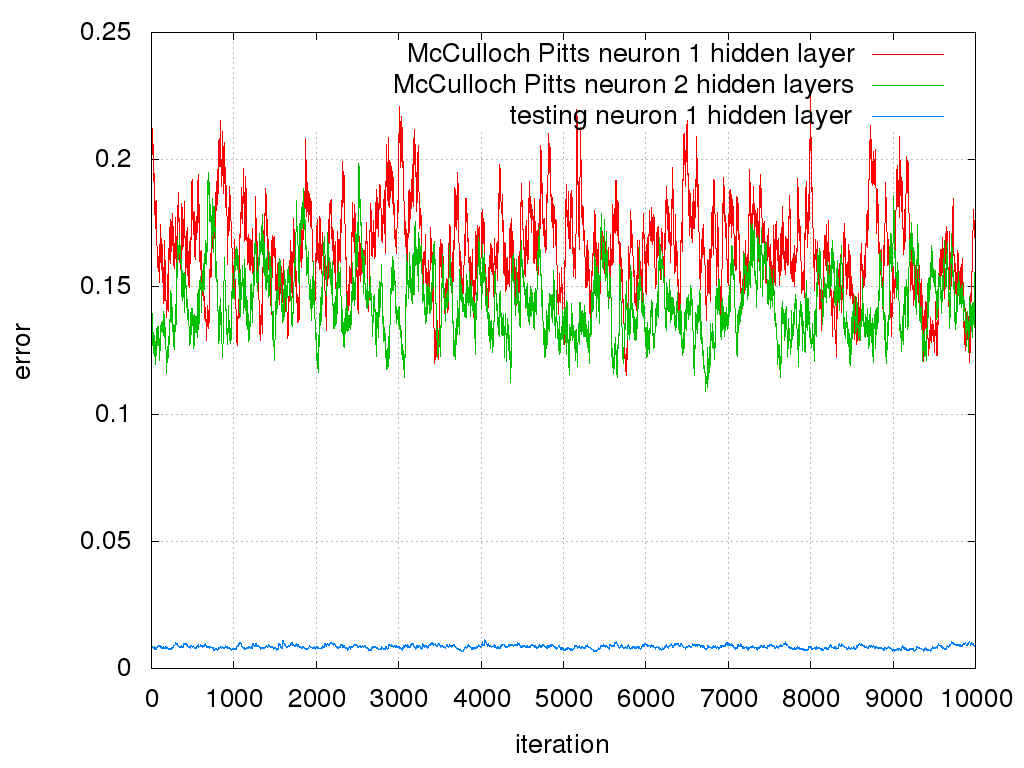
\includegraphics[width=2.5in]{multiplexer_result.png}
\caption{Multiplexer approximation error}
\label{multiplexer_result}
\end{figure}

\section{Conclusion}

In this paper we described neuron model improvement for
two inputs multiplications. Using only single hidden layer some
difficult problems for McCulloch-Pitts neural network can be solved.
It is necessary to normalise input and output vectors into  $\langle -1, 1 \rangle$ interval,
beacuse using high order powering in $\ref{multiplication_neuron}$ can be learning
algorithm unstable. \\
  Model has been tested on multiplexer problem learning using backpropagation.
  In future, more tests of these models are required.
  Some problems need to be solved : error backpropagation,
  hybrid learning using stochastic optimization and more application
  examples and tests.

\bibliographystyle{IEEEtran}
\bibliography{bib}

\begin{thebibliography}{4}

\bibitem{bib:Aproximation} Kolmogorov's Theorem,
http://neuron.eng.wayne.edu/tarek/MITbook/chap2/2\_3.html

\bibitem{bib:McCullochPitts} McCulloch Pitts neuron model,
http://www.mind.ilstu.edu/curriculum

\bibitem{bib:FeedForward} Comparsion of feedforward and reccurent neural network language models,
M. Sundermeyer, I. Oparin 2, J.-L. Gauvain, B. Freiberg 1, R. Schluter, H. Ney, 2013 IEEE

\bibitem{bib:Backpropagation} Backpropagation algorithm,
http://page.mi.fu-berlin.de/rojas/neural/chapter/K7.pdf

\end{thebibliography}



\end{document}
